\section{Results}

\subsection{Data}
As shown earlier, Figure \ref{fig:sampleData} is an example of some of the data we trained and tested with.
The training data consisted of 700 binary images for each character, with of different rotation and fonts.
The training data is a processed data set using our segmentation algorithm. This helps to keep our
training and testing data as realistic as possible. In addition, we also used images captures from the
tablet to perform periodic checks that our OCR was working properly.

\subsection{SVM}

\subsubsection{Training}
AS mentioned above, we utilized the different features to come up with a composite feature vector.
We took care to ensure that there was invariance with respect to rotation, illumination and size,
and that the algorithm did not take too long to run. We also experimented with Hough Transforms,
but it did not seem to suit our data, as it was projecting obvious lines. Skeletonising the characters
yielded little benefit if at all. We also experimented with using some expert-driven features \cite{frey}. We 
found this method from an online journal article about letter classification that 
spoke of a set of sixteen numerical attributes that when used to 
classify the 26 characters of the alphabet would completely separate the classes. 
These sixteen attributes were extracted after a pixel-by-pixel scan of the character. 
Included in these sixteen attributes are:\\
1. The horizontal position, counting pixels from the left edge of the image, of the center of the smallest 	rectangular box that can be drawn with all "on" pixels inside the box.\\
2. The vertical position, counting pixels from the bottom, of the above box.\\
3. The width, in pixels, of the box.\\
4. The height, in pixels, of the box.\\
5. The total number of "on" pixels in the character image.\\
6. The mean horizontal position of all "on" pixels relative to the center of the box and divided by the 	width of the box. This feature has a negative value if the image is "leftheavy" as would be the 	case for the letter L.\\
7. The mean vertical position of all "on" pixels relative to the center of the box and divided by the 	height of the box.\\
8. The mean squared value of the horizontal pixel distances as measured in 6 above. This attribute will 	have a higher value for images whose pixels are more widely separated in the horizontal 	direction as would be the case for the letters W or M.\\
9. The mean squared value of the vertical pixel distances as measured in 7 above.\\
10. The mean product of the horizontal and vertical distances for each "on" pixel as measured in 6 and 	7 above. This attribute has a positive value for diagonal lines that run from bottom left to top 	right and a negative value for diagonal lines from top left to bottom right.\\
11. The mean value of the squared horizontal distance times the vertical distance for each "on" pixel. 	This measures the correlation of the horizontal variance with the vertical position.\\
12. The mean value of the squared vertical distance times the horizontal distance for each "on" pixel. 	This measures the correlation of the vertical variance with the horizontal position.\\
13. The mean number of edges (an "on" pixel immediately to the right of either an "off" pixel or the 	image boundary) encountered when making systematic scans from left to right at all vertical 	positions within the box. This measure distinguishes between letters like "W" or "M" and letters 	like 'T' or "L."\\
14. The sum of the vertical positions of edges encountered as measured in 13 above. This feature will 	give a higher value if there are more edges at the top of the box, as in the letter "Y."\\
15. The mean number of edges (an "on" pixel immediately above either an "off" pixel or the image 	boundary) encountered when making systematic scans of the image from bottom to top over all 	horizontal positions within the box.\\
16. The sum of horizontal positions of edges encountered as measured in 15 above
The best accuracy that was found using the sixteen attribute set as the feature selector was 72.45\%, 
which isn't nearly as accurate as the other combinations of features. Because of these slow processes, 
training the images takes a very long time along the lines of four to five hours. While training only needs 
to be done once in order to use the Support Vector Machine, the testing also is not quick at all and takes 
awhile to calculate and compare the images' attributes making this process a very slow one.  
One solution we considered is removing and adjusting some of the attributes as to speed up the 
process while still maintaining the accuracy of this method.  Since attributes thirteen through 
sixteen were the main contributors to the speed issue, we chose to remove them and try to see if 
the accuracy would still remain the same.  When testing on the same test data as the original data, 
the twelve attribute set accuracy was greatly reduced from the set using all sixteen attributes.  
The accuracy we got from the twelve attribute set was 48.15\%.  
These results may have occurred because of many reasons.  
The reason for errors when using the sixteen attribute set seem to be 
from rotation, illumination, and the various fonts used in the simulation.  
The rotation will affect many of the attributes such as the edges and the horizontal 
and vertical positions which will throw off the strength of the correlation between each 
character.  With the illumination involved in the image, the binary interpretation of the 
image would definitely change the image because illumination would change multiple areas that 
were “off” pixels into “on” pixels. \\

Finally, we did further analysis on using differnt combinations, as well as differnt feature vector length, 
of the previous elaborated features, e.g. fourier descriptors etc. 
Training was sped up using the ECE servers. (8 cores were able to train 25200 images in 2 hours).

\subsubsection{Results}
\begin{figure}[h]
		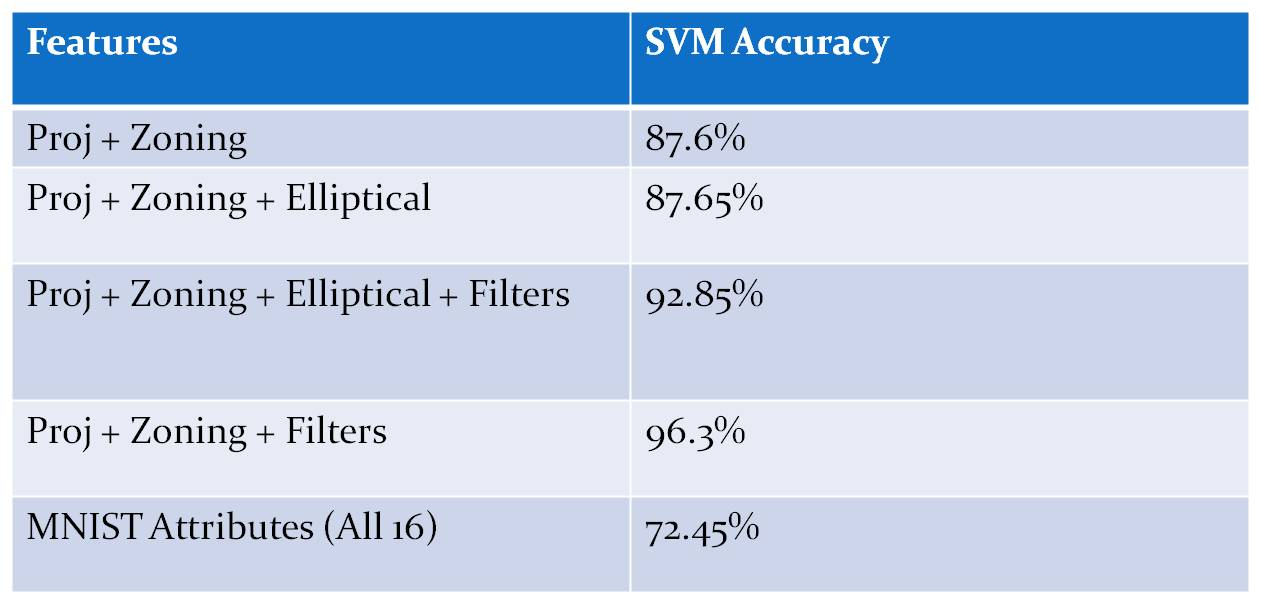
\includegraphics[scale=0.80]{svmResults.jpg}\\
		\caption{Figure showing the accuracy using different features for our SVM}
		\label{fig:svmresults}
\end{figure}
Figure \ref{fig:svmresults} shows that the filters together with zoning seem to be most effective.
In this case, we had used a filterbank of 6 different orientations of Gabor filters,
and combined with zoning, seems to have given the best accruacy at 96.3\%. This is probably due
to the gabor filter's effectiveness in detecing the differnt edges. Furthermore, research has also
shown that typically the sparse codes basis for natural images, tend to have gabor like features.
In this sense, our results confirm their findings. However, it is very computationally expensive
to run the characters through the filterbank and our processing time suffers for it.


\subsection{Correlation Filters}
Another optical character recognition method we used was correlation filters. 
Unlike SVMs, correlation filters use templates based on far fewer training 
images to compare to the input image. While less robust than SVMs, we found 
that the correlation filters were much easier and quicker to train at the 
expense of requiring one filter per letter, font, and greater than \~5 degrees 
of rotation. Because we initially focused on recognizing only capital letters 
in one font, however, the results showed high accuracy, often categorizing all 
26 input characters correctly.\\
All of the filters were first coded in Matlab for testing, and only once the most 
steadily accurate filtering algorithm was confirmed did we attempt to convert the 
code into a language able to be handled by the Android tablet. Unfortunately, the 
code conversion was far more complicated than we anticipated, and only the 
simplified versions of the correlation filters were able to be implemented. We did, 
however, use the Android server/client system to send images through the Matlab 
code to ensure the filters would work if the tablet could run the code.

\subsubsection{Simple Correlation}

\begin{figure}[h]
		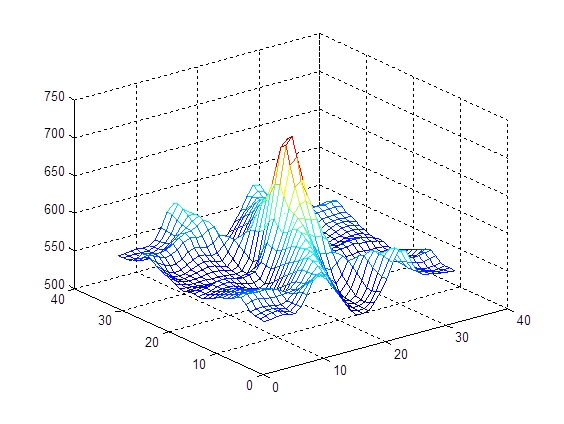
\includegraphics[scale=0.80]{corr.jpg}\\
		\caption{Simple Correlation Energy Plane between input 'A' and 'A' filter.}
		\label{fig:corr}
\end{figure}


\begin{equation}
\label{eqn332}
Correlation = ifft2(fft2(input).*conj(fft2(filter)));
\end{equation}

The first correlation filter we implemented worked off a 
single template image ('filter', in \eqref{eqn332})
for the correlation equation (\eqref{eqn332} documents the Matlab 
code used). While we initially had some trouble generating the 
appropriate figures, we soon learned how similar the training 
and testing images needed to be in order to achieve pleasing results 
(see figure \ref{fig:corr} for an example). Once the code was modified, 
the simple correlation filters showed an average of an 89% success rate 
across over 100 tested characters, though our final testing set for the
demonstration yielded a 0\% success rate across 26 
capital-letter inputs. While just under half of the initial testing 
characters were derived from the same images used to generate the training 
data, we did not detect a noticeable difference across testing sets. Further, 
the tested characters were passed through different filters than the training 
characters to provide noise and rotation in order to ensure variance between 
sets. As our final testing set provided noisier inputs to thoroughly test the 
robustness of the various OCR methods, we were not surprised to find that the 
simple correlation filter had such a low accuracy.\\
\\
The same training and testing data was used for all of the following 
correlation filter algorithms. While we would have liked to test on a 
larger number of inputs, the illumination greatly affected the accuracy 
of the filters, leaving us with far less usable images than desired. 
Though more rigorous testing may result in slightly lower success rates, 
we are confident that the difference would not contradict the general 
overview of our results. Further, because 26 filters could be generated 
in a matter of seconds, tweaking the noise filters before correlation 
allowed us to increase categorization success quickly depending on the 
location in which the input image was captured.

\subsubsection{Equal Correlation Peak - Synthetic Discriminant Function}

\begin{figure}[h]
		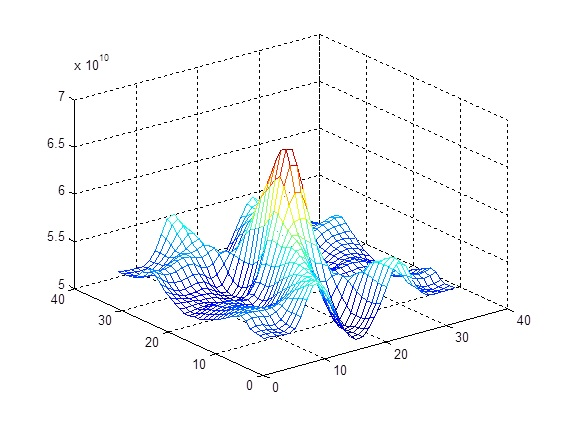
\includegraphics[scale=0.80]{corr1.jpg}\\
		\caption{ ECP-SDF Correlation Energy Plane between input ‘A’ and ‘A’ filter}
		\label{fig:corr1}
\end{figure}

\begin{equation}
\label{eqn333}
H = X(X+X)^{-1} u
\end{equation}

The next filter we coded and tested was an ECP-SDF. The main difference between
this filter - and the two following - and the simple correlation filter is that
these filter algorithms allow more than one training image 
to generate the template for correlation. In order to accomplish this, 
the Fourier transform of 'filter' in \eqref{eqn332} is replaced with \textbf{H}, an 
aggregate vector of the training images in the frequency domain \textbf{(X)}, as 
described in \eqref{eqn333} Further, this and the following filters allow 
training images to be weighted via u, a one-dimensional vector containing 
1s for a positive correlation and -1s for the opposite. While this would 
mainly be used to differentiate similar characters from one another, i.e. 
'E' and 'F', we found that too many training images corrupted the filters, 
preventing them from working as intended.\\

Surprisingly, despite the seeming increase in robustness of the 
pre-correlation algorithm, the ECP-SDF performed more poorly than 
the simple correlation filter, with an average accuracy of around 
70\% over the initial testing set. Despite the large decrease in successful 
categorizations in the testing sets, the correlation energy planes are 
hardly distinguishable from those of the simple correlation filters (figure \ref{fig:corr1}), 
and the ECP-SDF algorithm worked significantly better than the simple filters over
the final demonstration inputs, achieving a 61.5\% categorization accuracy there.
\subsubsection{Minimum Average Correlation Energy Filter}

\begin{figure}[h]
		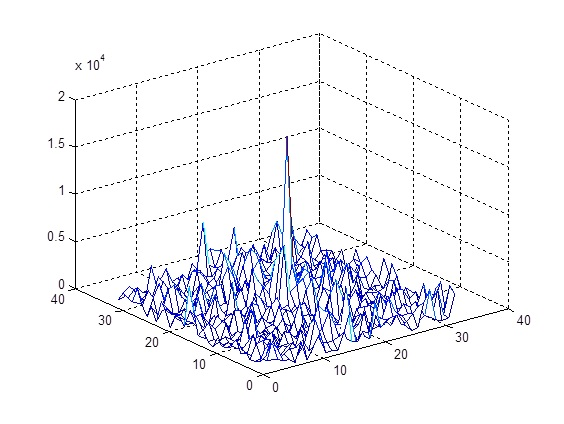
\includegraphics[scale=0.80]{corr2.jpg}\\
		\caption{MACE Filter Correlation Energy Plane between input ‘B’ and ‘B’ filter.}
		\label{fig:corr2}
\end{figure}

\begin{equation}
\label{eqn3341}
H = D^{-1}X(X+D^{-1}X)^{-1} u
\end{equation}

\begin{equation}
\label{eqn3342}
D_{i}(k, k) = |X_{i}(k)|^{2}
\end{equation}

The MACE filter alters the equation for H \eqref{eqn3341} by introducing D \eqref{eqn3342}, 
a diagonal matrix of the power spectrum of the training images. In Matlab, this was done 
by averaging the magnitude square of the training images in the frequency domain.

As seen in figure \ref{fig:corr2}, the MACE filter correlation energy plane differs 
dramatically from those of the previous two correlation filters. The more 
pronounced peak yields far better results as well, achieving an average accuracy 
of 100\% over the initial testing sets, and 88.5\% categorization accuracy over the 
final demonstration set.

Because of the success rate, we selected the MACE filter for 
the majority of the debugging and testing of the various PSR 
algorithms (see PSR Section). This was mostly done before the 
final demonstration set was generated, though, which partially 
helps to explain our decision.

\subsubsection{Optimal Trade-Off Synthetic Discriminant Function}
\begin{figure}[h]
		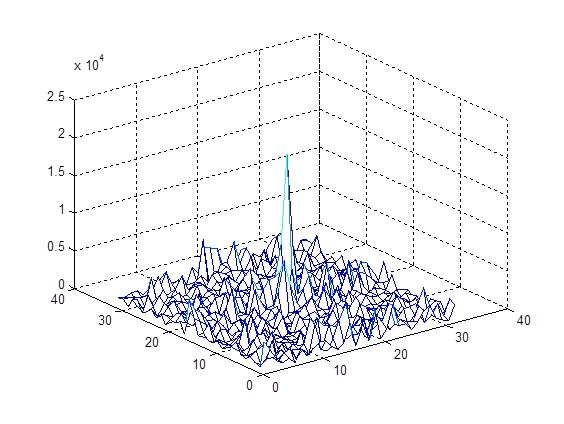
\includegraphics[scale=0.80]{corr3.jpg}\\
		\caption{OTSDF Correlation Energy Plan between input ‘B’ and ‘B’ filter.}
		\label{fig:corr3}
\end{figure}
The final filter we coded and tested was the OTSDF. 
While very similar to the MACE filter (see figure \ref{fig:corr3}), 
the OTSDF alters \textbf{D} to handle noise \eqref{eqn3351}. In the equation, $\alpha$ 
can be selected based on the amount of noise to train for, and $\beta$ simply 
depends on $\alpha$ \eqref{eqn3352}. Though we initially tested with $\alpha = 0.99$, we 
found that $\alpha = 0.75$ accounted for our input better, especially for the final 
demonstration data set.

\begin{equation}
\label{eqn3351}
D_{new} = \alpha D_{MACE} + \beta I
\end{equation}

\begin{equation}
\label{eqn3352}
\beta = \sqrt{(1 - \alpha^{2}}
\end{equation}

In testing, the OTSDF averaged 100\% accuracy with the same testing data sets as the other three correlation filters, but due to pre-processing, the value of $\alpha$ did not affect results. However, during our preparation for the demonstration, we found that the OTSDF, while more accurate than the MACE filter, repeatedly categorized 'F' as 'E'. This was when we learned of the usefulness of the change to \textbf{D}; blurring the training images to add noise after pre-processing, along with an adjusted $\alpha$, allowed for 100\% correct categorization over the final demonstration inputs. \\
Because of the accuracy and superior robustness of the OTSDF, while we were unable to convert the Matlab code entirely to the Android application, we realize this is the most promising of the correlation filters.

\subsubsection{Peak-Sidelobe Ratio}
As a way of measuring the success of a correlation (\textbf{C}), we computed the PSR of the correlation energy planes. This allowed us to quickly tell which filter matched each input best, allowing the categorization of each character to process smoothly. Initially, we calculated a simplified version of the PSR in Matlab \eqref{eqn336} to compare the various correlation filters. While this computation worked for debugging, a more accurate algorithm was necessary.

\begin{equation}
\label{eqn336}
PSR_{simple} = (max(C) - mean(C)) / std(C);
\end{equation}

In order to more properly calculate the PSR, by definition, we needed to take the mean and standard deviation of the sidelobe of the correlation energy plane. To do so, we essentially masked a 5x5 area of the correlation centered on the maximum value, and used the rest of the values for the sidelobe. While this was not necessarily the best way to compute the PSR, we saw a noticeable difference in our results (figure \ref{fig:alexTable}). Unfortunately, the masking process did not convert to the Android easily, but we found that the simplified PSR worked to a reasonable extent, at least allowing us to compare the correlation filter method of OCR to the other processes.

\begin{figure}[!]
		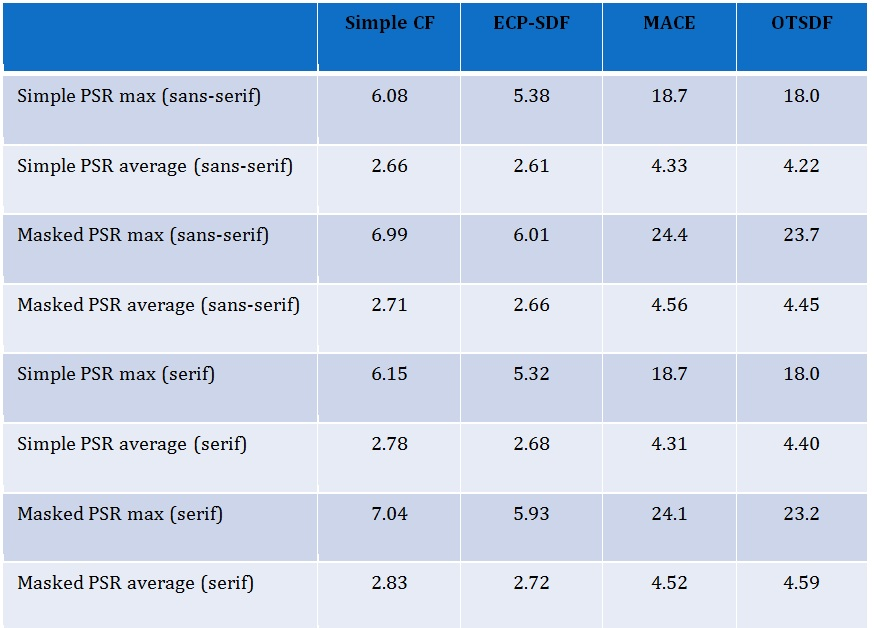
\includegraphics[scale=0.66]{alexTable.jpg}\\
		\caption{Simplified and masked PSR data for each correlation filter across serif and sans-serif testing sets.}
		\label{fig:alexTable}
\end{figure}